\documentclass[12pt,a4paper]{article}
\usepackage{lmodern}

\usepackage{amssymb,amsmath}
\usepackage{ifxetex,ifluatex}
\usepackage{fixltx2e} % provides \textsubscript
\ifnum 0\ifxetex 1\fi\ifluatex 1\fi=0 % if pdftex
  \usepackage[T1]{fontenc}
  \usepackage[utf8]{inputenc}
\else % if luatex or xelatex
  \ifxetex
    \usepackage{mathspec}
    \usepackage{xltxtra,xunicode}
  \else
    \usepackage{fontspec}
  \fi
  \defaultfontfeatures{Mapping=tex-text,Scale=MatchLowercase}
  \newcommand{\euro}{€}
\fi
% use upquote if available, for straight quotes in verbatim environments
\IfFileExists{upquote.sty}{\usepackage{upquote}}{}
% use microtype if available
\IfFileExists{microtype.sty}{%
\usepackage{microtype}
\UseMicrotypeSet[protrusion]{basicmath} % disable protrusion for tt fonts
}{}
\usepackage[lmargin = 5cm,rmargin = 2.5cm,tmargin = 2.5cm,bmargin = 2.5cm]{geometry}

% Figure Placement:
\usepackage{float}
\let\origfigure\figure
\let\endorigfigure\endfigure
\renewenvironment{figure}[1][2] {
    \expandafter\origfigure\expandafter[H]
} {
    \endorigfigure
}

%%%% Jens %%%%
\DeclareMathOperator*{\argmax}{arg\,max}
\DeclareMathOperator*{\argmin}{arg\,min}

\usepackage{numprint}
\npthousandsep{\,}

%% citation setup
\usepackage{csquotes}

\usepackage[backend=biber, maxbibnames = 99, style = apa]{biblatex}
\setlength\bibitemsep{1.5\itemsep}
\addbibresource{R_packages.bib}
\bibliography{references.bib}
\usepackage{graphicx}
\makeatletter
\def\maxwidth{\ifdim\Gin@nat@width>\linewidth\linewidth\else\Gin@nat@width\fi}
\def\maxheight{\ifdim\Gin@nat@height>\textheight\textheight\else\Gin@nat@height\fi}
\makeatother
% Scale images if necessary, so that they will not overflow the page
% margins by default, and it is still possible to overwrite the defaults
% using explicit options in \includegraphics[width, height, ...]{}
\setkeys{Gin}{width=\maxwidth,height=\maxheight,keepaspectratio}
\ifxetex
  \usepackage[setpagesize=false, % page size defined by xetex
              unicode=false, % unicode breaks when used with xetex
              xetex]{hyperref}
\else
  \usepackage[unicode=true, linktocpage = TRUE]{hyperref}
\fi
\hypersetup{breaklinks=true,
            bookmarks=true,
            pdfauthor={Jens Klenke},
            pdftitle={Bayes Seminar},
            colorlinks=true,
            citecolor=black,
            urlcolor=black,
            linkcolor=black,
            pdfborder={0 0 0}}
\urlstyle{same}  % don't use monospace font for urls
\setlength{\parindent}{0pt}
\setlength{\parskip}{6pt plus 2pt minus 1pt}
\setlength{\emergencystretch}{3em}  % prevent overfull lines
\setcounter{secnumdepth}{5}

%%% Use protect on footnotes to avoid problems with footnotes in titles
\let\rmarkdownfootnote\footnote%
\def\footnote{\protect\rmarkdownfootnote}

%%% Change title format to be more compact
\usepackage{titling}

% Create subtitle command for use in maketitle
\newcommand{\subtitle}[1]{
  \posttitle{
    \begin{center}\large#1\end{center}
    }
}

\setlength{\droptitle}{-2em}
  \title{Bayes Seminar}
  \pretitle{\vspace{\droptitle}\centering\huge}
  \posttitle{\par}
\subtitle{Advanced R for Econometricians}
  \author{Jens Klenke}
  \preauthor{\centering\large\emph}
  \postauthor{\par}
  \predate{\centering\large\emph}
  \postdate{\par}
  \date{today}

\usepackage{booktabs}
\usepackage{longtable}
\usepackage{array}
\usepackage{multirow}
\usepackage{wrapfig}
\usepackage{float}
\usepackage{colortbl}
\usepackage{pdflscape}
\usepackage{tabu}
\usepackage{threeparttable}
\usepackage{threeparttablex}
\usepackage[normalem]{ulem}
\usepackage{makecell}
\usepackage{xcolor}

%% linespread settings

\usepackage{setspace}

\onehalfspacing

% Language Setup

\usepackage{ifthen}
\usepackage{iflang}
\usepackage[super]{nth}
\usepackage[ngerman, english]{babel}

%Acronyms
\usepackage[printonlyused, withpage, nohyperlinks]{acronym}
\usepackage{changepage}

% Multicols for the Title page
\usepackage{multicol}

\begin{document}

\selectlanguage{english}

%%%%%%%%%%%%%% Jens %%%%%
\numberwithin{equation}{section}


%\maketitle

\begin{titlepage}
  \noindent\begin{minipage}{0.6\textwidth}
	  \IfLanguageName{english}{University of Duisburg-Essen}{Universität Duisburg-Essen}\\
	  \IfLanguageName{english}{Faculty of Business Administration and Economics}{Fakultät für Wirtschaftswissensschaften}\\
	  \IfLanguageName{english}{Chair of Econometrics}{Lehrstuhl für Ökonometrie}\\
  \end{minipage}
	\begin{minipage}{0.4\textwidth}
	  \begin{flushright}
  	  \vspace{-0.5cm}
      \IfLanguageName{english}{\includegraphics*[width=5cm]{Includes/duelogo_en.png}}{\includegraphics*[width=5cm]{Includes/duelogo_de.png}}
	  \end{flushright}
	\end{minipage}
  \\
  \vspace{1.5cm}
  \begin{center}
  \huge{Bayes Seminar}\\
  \vspace{.25cm}
  \Large{Advanced R for Econometricians}\\
  \vspace{0.5cm}
  \large{Seminar Paper}\\
  \vspace{1cm}
  \large{  \IfLanguageName{english}{Submitted to the Faculty of \\ Ökonometrie  \\at the \\University of Duisburg-Essen}{Vorgelegt der \\Fakultät für Wirtschaftswissenschaften der \\ Universität Duisburg-Essen}\\}
  \vspace{0.75cm}
  \large{\IfLanguageName{english}{from:}{von:}}\\
  \vspace{0.5cm}
  Jens Klenke\\
  \end{center}
  %\vspace{2cm}
  \vfill
  \hrulefill

  \noindent\begin{minipage}[t]{0.3\textwidth}
  \IfLanguageName{english}{Reviewer:}{Erstgutachter:}
  \end{minipage}
  \begin{minipage}[t]{0.7\textwidth}
  \hspace{1cm}Christoph Hanck
  \end{minipage}

  \noindent\begin{minipage}[t]{0.3\textwidth}
  \IfLanguageName{english}{Deadline:}{Abgabefrist:}
  \end{minipage}
  \begin{minipage}[t]{0.7\textwidth}
  \hspace{1cm}Jan.~17th 2020
  \end{minipage}

  \hrulefill

  \begin{multicols}{2}

  Name:

  Matriculation Number:

  E-Mail:

  Study Path:

  Semester:

  Graduation (est.):
 
  \columnbreak

  Jens Klenke

  3071594
  
  jens.klenke@stud.uni-due.de

  M.Sc. Economics

  \nth{5}

  Winter Term 2020

	\end{multicols}

\end{titlepage}

\newgeometry{top=2cm, left = 5cm, right = 2.5cm, bottom = 2.5cm}


\pagenumbering{Roman}
{
\hypersetup{linkcolor=black}

\setcounter{tocdepth}{3}
\tableofcontents
}

\newpage
\listoffigures
\addcontentsline{toc}{section}{List of Figures}

%\newpage
\listoftables
\addcontentsline{toc}{section}{List of Tables}

\section*{List of Abbreviations}
\addcontentsline{toc}{section}{List of Abbreviations}

\begin{adjustwidth}{1.5em}{0pt}

\begin{acronym}[dummyyyy]
 \acro{bagging}{Bootstrap Aggregation}
 \acro{LASSO}{Least Absolute Shrinkage and Selection Operator}
 \acro{pcr}{Principal Components Regression}
 \acro{pls}{Partial Least Squares}
 \acro{RMSE}{Root Mean Squared Error}
 \acro{MCMC}{Markov chain Monte Carlo} 
 \acro{i.i.d.}{independent and identically distributed}
 \acroplural{LRG}[LRG]{längefristige Refinanzierungsgeschäfte}

%Falls eine Abkürzung in der Mehrzahl nicht einfach auf "s" endet muss das speziell eingestellt werden.
% \acro{slmtA}{super lange mega tolle Abkürzung} %Einzahl
 %\acroplural{slmtA}[slmtAs]{super lange mega tolle Abkürzungen} %Mehrzahl
 \acro{dummyyyy}{dummyyy}
\end{acronym}

\end{adjustwidth}

\restoregeometry

\newpage
\pagenumbering{arabic}
\hypertarget{introduction}{%
\section{Introduction}\label{introduction}}

In recent years, the \ac{LASSO} method of TIBSHIRANI has emerged as an
alternative to ordinary least squares estimation. The success of the
method is mainly due to its ability to perform both variable selection
and estimation. As already Tibshirani pointed out in his original paper
the standard \ac{LASSO} model can be interpreted as a linear regression
with a Laplace prior. PARK and CASELLA where the first to implement the
Bayesian l\ac{LASSO} \textgreater\textgreater using a conditional
Laplace prior specification\textless\textless.

Our goal is to compare the result of the Bayesian \ac{LASSO} with normal
\ac{LASSO} method and an ordinary least square estimation. The focus is
particularly on the number of non-significant parameters in the linear
model or, in case of the \acp{LASSO} the parameters equal to zero.

\newpage

\hypertarget{theory-of-bayesian-inference}{%
\section{Theory of Bayesian
inference}\label{theory-of-bayesian-inference}}

The Bayesian (inference) statistics based on the Bayes' theorem for
events.

\begin{align}
\label{eq:bayes_theorem}
  P(A | B) = \dfrac{P (B | A) P(A)}{P(B)}
\end{align}

For Bayesian statistics the event theorem gets \eqref{eq:bayes_theorem}
rewritten to apply it to densities. Where \(\pi (\theta)\) is the prior
distribution - which could be gained from prior research or knowledge,
\(f(y | \theta )\) is the likelihood function, and \(\pi (\theta| y)\)
is the posterior distribution, we then get the following.

\begin{align}
\label{eq:bayes_dens}
  \pi (\theta | y) = \dfrac{f(y | \theta) \pi(\theta)}{f(y)}
\end{align}

From \eqref{eq:bayes_dens} the advantages and disadvantages of Bayesian
statistics compared to frequentist statistics can directly be retrieved.
One major adavantage is that the Bayesian approach can account for prior
knowledge and points out a philosophical difference to the frequentist
approach - that the obtained data stands not alone. Another, key
difference and advantage is that in the Bayesian world the computation
are made with distributions and this leads to a better information level
than just the computation of the first and second moment. The
computation of distributions are also the greatest disadvantages or more
neutral the biggest problem of the Bayesian approach because in high
dimensional problems the computation takes a lot of times or is
sometimes even not possible. A solution to that is that with newer and
better computers it is possible to simulate the integrals with a
\ac{MCMC} method. GHOSH

\newpage

\hypertarget{data-description}{%
\section{Data description}\label{data-description}}

We collected the data from the online database platform \emph{kaggel.}
\autocite{leone_fifa_2020} ZITATE The dataset included 6 years of data
for all players which where included in the soccer simulation game
\emph{FIFA} from \emph{EA Sports}. We dicided to just keep the data for
2019 and 2020. The Data for 2019 contains 17538 datapoints will be used
for the estimation of the differen models whereas the 2020 data with
18028 will be used to compare the quality of the models with an out of
sample \ac{RMSE}.

\textcite{leone_fifa_2020}

A fundamental problem of the data set was that goalkeepers are
systematically rated differently than field players. Therefore, in the
subcategories of \emph{overall} all field player categories were
assigned to NAs. Conversely, all field players have NAs in all
goalkeeper categories. Because the algorithm of \ac{LASSO} in R cannot
handle NAs, they are set to zero for all models.

It is not very realistic that a fielder has no values in the goalkeeper
categories and vice versa. However, it can be argued, at least for
outfield players, that goalkeeper attributes play no role in determining
market values. This argumentation does not seem to hold for goalkeepers,
at least passing can be assumed to be an influential variable for the
market value. Nevertheless, due to the lack of alternatives, all NAs
have been replaced by zero.

\begin{table}[!h]

\caption{\label{tab:unnamed-chunk-3}\label{tab:sum} Summary of some important variables for the 2019 FIFA edition}
\centering
\begin{tabular}[t]{lllrlrr}
\toprule
 & year &  & N &   & mean & sd\\
\midrule
\rowcolor{gray!6}  value\_eur & 2019 &  & 17 538 &  & 2 473 043.68 & 5 674 963.22\\
 & 2020 &  & 18 028 &  & 2 518 484.58 & 5 616 359.21\\
\rowcolor{gray!6}  wage\_eur & 2019 &  & 17 538 &  & 10 085.87 & 22 448.70\\
 & 2020 &  & 18 028 &  & 9 584.81 & 21 470.29\\
\rowcolor{gray!6}  overall & 2019 &  & 17 538 &  & 66.23 & 7.01\\
 & 2020 &  & 18 028 &  & 66.21 & 6.95\\
\rowcolor{gray!6}  age & 2019 &  & 17 538 &  & 25.17 & 4.64\\
 & 2020 &  & 18 028 &  & 25.23 & 4.63\\
\rowcolor{gray!6}  potential & 2019 &  & 17 538 &  & 71.40 & 6.15\\
 & 2020 &  & 18 028 &  & 71.56 & 6.14\\
\bottomrule
\end{tabular}
\end{table}

As one can see in Table \ref{tab:sum} the differences between the
editions for the most important variables are considerable small. For
example, from 2019 to 2020 the mean player \emph{value} (response
variable) increased by 4.54e+04 which is about 1.8 per cent or 0.01
standard deviations. Simular results are observabel for the probly most
importanten righthand variables \emph{wage} and \emph{overall} with a
difference in the means of -0.02 and -0.003 standard deviations between
2019 and 2020.

\begin{figure}
\centering
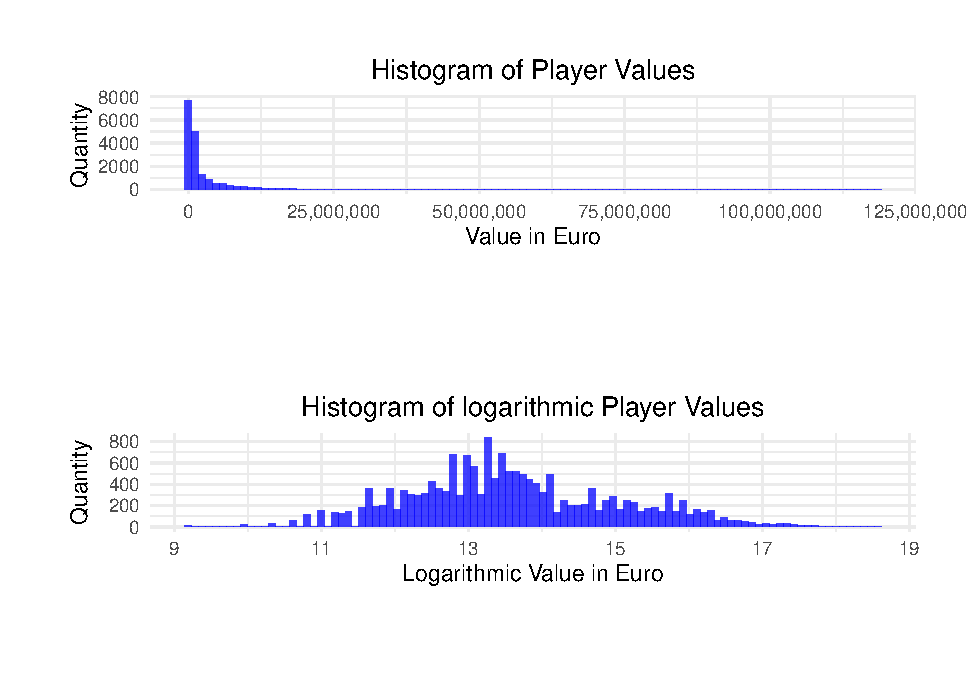
\includegraphics{term_paper_bayes_files/figure-latex/fig1-1.pdf}
\caption{\label{fig:hist_1} Histograms of player values and log player
values}
\end{figure}

As can be seen for the variable value in Figure \ref{fig:hist_1}, this
relatively strong right-skew is distributed, a similar pattern can be
observed for the variable wage. Since we also estimate a linear model
and this often leads to non-normally distributed residuals, these were
logarithmized.

\newpage

\hypertarget{models-used}{%
\section{Models used}\label{models-used}}

To compare the Bayesian \ac{LASSO} we will analyse the data also with a
linear multivariate model, and the frequentist \ac{LASSO}. We wil start
with the linear model and will modifie the model equations step by step
forward the bayesian version.

\hypertarget{linear-model}{%
\subsection{Linear Model}\label{linear-model}}

The frequentist multivariate regression model has the follwing model
equation.

\begin{align}
\label{eq:lm}
\pmb{Y = \beta_0 + X \beta} + \pmb{\epsilon}
\end{align}

Where \(\pmb{y}\) is the \(n \times 1\) response vector, \(\pmb{X}\) is
the \(n \times p\) matrix of regressors and, \(\pmb{\epsilon}\) is the
\(n \times 1\) vecotr of \ac{i.i.d.} errors with mean 0 and unknown
variance \(\sigma^2\). The coefficient will be estimated by the ordinary
least square method, which means that \(\pmb{\beta}\) should be chosen
so that the \emph{Euclidean norm}
\(\left( || \mathbf{y - X\beta} ||_2 \right)\) is minimal. This yields
in the conditon for the estimation of coefficients:

\begin{align}
\label{eq:lm_con}
 \hat{\pmb{\beta}} = \argmin_{ \pmb{\beta}} (\pmb{y - \beta_0 - X  \beta})^T (\pmb{y - \beta_0 - X  \beta})
\end{align}

\hypertarget{section}{%
\subsection{\texorpdfstring{\acf{LASSO}}{}}\label{section}}

In the \ac{LASSO} method the model equation is the same as the equation
for the multivariate but the condition for the optimization of the
estimators in equation \eqref{eq:lm_con} has an additional punishment
term. Which leads to the optimazation of:

\begin{align}
\label{eq:la_con}
\hat{\pmb{\beta}} = \argmin_{\pmb{\beta}}  \left( \pmb{y - X \beta} \right)^T \left( \pmb{y - X \beta} \right) + \lambda \sum_{i = 1}^{p} |\beta_j|
\end{align}

for some \(\lambda \geq 0\). This method is also often referred to as
\(L_1\) -penalized least squares estimation.

Already in his original paper \textcite{tibshirani_regression_1996} has
pointed out the possibility that his methods can also be interpreted
Bayesian. The LASSO estimates can be considered as posterior mode
estimates with a double-exponential Laplace prior .

\hypertarget{bayesian-lasso}{%
\subsection{Bayesian Lasso}\label{bayesian-lasso}}

\textcite{park_bayesian_2008} considered a fully Bayesian approach using
a conditional Laplace prior of the form

\begin{align} 
\label{eq:la_bay_prior}
 \pi \left( \beta | \sigma^2 \right)   = \prod_{j = 1}^{p} \dfrac{\lambda}{2 \sqrt{\sigma^e}} e^{\dfrac{- \lambda |\beta_j |}{\sqrt{\sigma^2}}} 
\end{align}

\autocite{park_bayesian_2008}

\hypertarget{gibbs-sampler}{%
\subsubsection{Gibbs Sampler}\label{gibbs-sampler}}

\hypertarget{estimation-of-the-bayesian-lasso}{%
\section{Estimation of the Bayesian
Lasso}\label{estimation-of-the-bayesian-lasso}}

\hypertarget{posteriod-based-estimation-and-prediction}{%
\section{Posteriod-based Estimation and
prediction}\label{posteriod-based-estimation-and-prediction}}

\hypertarget{residuals-and-sensitive-analysis}{%
\section{Residuals and Sensitive
Analysis}\label{residuals-and-sensitive-analysis}}

\hypertarget{discussion-and-further-research}{%
\section{Discussion and further
research}\label{discussion-and-further-research}}

\newpage

\renewcommand*{\mkbibnamefamily}[1]{\textbf{#1}}
\renewcommand*{\mkbibnamegiven}[1]{\textbf{#1}}
\renewcommand*{\mkbibnameprefix}[1]{\textbf{#1}}
\renewcommand*{\mkbibnamesuffix}[1]{\textbf{#1}}
\printbibliography[title=References]



\newpage
\textbf{Eidesstattliche Versicherung}

\bigskip

Ich versichere an Eides statt durch meine Unterschrift, dass ich die vorstehende Arbeit selbständig und ohne fremde Hilfe angefertigt und alle Stellen, die ich wörtlich oder annähernd wörtlich aus Veröffentlichungen entnommen habe, als solche kenntlich gemacht habe, mich auch keiner anderen als der angegebenen Literatur oder sonstiger Hilfsmittel bedient habe. Die Arbeit hat in dieser oder ähnlicher Form noch keiner anderen Prüfungsbehörde vorgelegen.

\vspace{1cm}
\rule{0pt}{2\baselineskip} %
\par\noindent\makebox[2.25in]{\indent Essen, den \hrulefill} \hfill\makebox[2.25in]{\hrulefill}%
\par\noindent\makebox[2.25in][l]{} \hfill\makebox[2.25in][c]{Jens Klenke}%


\end{document}
